%!TeX program = xelatex
% VizDOM - Tài liệu kiến trúc arc42 (Tiếng Việt). Biên dịch bằng XeLaTeX (xem README.md).
% Overleaf: Menu -> Settings -> Compiler -> XeLaTeX (fontspec cần XeTeX/LuaTeX).
\documentclass[11pt,a4paper]{report}

\usepackage{fontspec}
\usepackage[vietnamese]{babel}
\usepackage{microtype}
\usepackage{geometry}
\geometry{margin=2.4cm}
\usepackage{graphicx}
\usepackage{booktabs}
\usepackage{array}
\usepackage{longtable}
\usepackage{caption}
\usepackage{enumitem}
\usepackage{xcolor}
\usepackage[hidelinks]{hyperref}
\usepackage{float}
\usepackage{titlesec}

\graphicspath{{figures/}}
\newcommand{\code}[1]{\texttt{#1}}
\newcommand{\req}[1]{\textbf{#1}}
\setlength{\parskip}{0.4em}
\setlength{\parindent}{0pt}
\setlength{\tabcolsep}{4pt}
\renewcommand{\arraystretch}{1.25}

% Các phần của arc42 được trình bày dưới dạng chương; giữ cách đánh số "N".
\titleformat{\chapter}[hang]{\normalfont\huge\bfseries}{\thechapter}{1em}{}
\titlespacing*{\chapter}{0pt}{0pt}{1em}

\title{\textbf{VizDOM --- Tài liệu Kiến trúc}\\[0.3em]
\large theo mẫu arc42}
\author{Nguyễn Huỳnh Trí Cường\\
\small Đồ án ứng dụng cao học (Khoa học máy tính) --- Trường Đại học Khoa học Tự nhiên, TP. Hồ Chí Minh\\
\small Khoa Công nghệ Thông tin\\
\small Giảng viên hướng dẫn: PGS. TS. Nguyễn Văn Vũ}
\date{2026 --- Phiên bản 1.0}

\begin{document}
\maketitle

\begin{abstract}
\noindent Tài liệu này mô tả kiến trúc phần mềm của \textbf{VizDOM}, một hệ thống tái tạo
Mô hình Đối tượng Tài liệu (Document Object Model --- DOM) tương tự UI Automator từ
ảnh chụp giao diện GUI, qua đó hỗ trợ tự động hóa kiểm thử cho các ứng dụng không cung
cấp cây accessibility. Tài liệu tuân theo mẫu arc42 và kỷ luật ra quyết định kiến trúc
SWA (drivers~$\rightarrow$~giải pháp~$\rightarrow$~tài liệu hóa~$\rightarrow$~xác minh).
Nguyên tắc xuyên suốt là khả năng truy vết: mọi lựa chọn có ý nghĩa kiến trúc đều được
liên kết với một driver đã được xếp hạng và, khi có thể, với bằng chứng có thể đo lường.
VizDOM là đồ án ứng dụng theo Phương thức 3; kiến trúc ưu tiên khả năng sửa đổi
(các cơ chế detection/capture/actuation có thể thay thế), khả năng triển khai
(mỗi chức năng có thể chạy cục bộ hoặc dưới dạng dịch vụ gRPC từ xa) và khả năng kiểm thử,
thay vì tập trung vào tính mới của thuật toán.
\end{abstract}

\tableofcontents

% =====================================================================
\chapter{Giới thiệu và Mục tiêu}
% =====================================================================
VizDOM chuyển đổi một \emph{ảnh chụp màn hình} GUI thành một \emph{Visual DOM} có cấu
trúc và có thể truy vấn --- bao gồm biên phần tử, role, text, label, locator và cấu trúc
phân cấp --- bằng computer vision kết hợp với một mô hình ngôn ngữ/thị giác nhỏ, sau đó
cung cấp DOM này cho test framework. Hệ thống hướng đến các ứng dụng mà cây accessibility
của nền tảng (Android UI~Automator, Windows~UIA, web DOM) không tồn tại hoặc không đáng
tin cậy: các UI desktop được custom-render bằng Qt/QML, OpenGL hoặc game engine; HMI
nhúng và công nghiệp; cũng như màn hình được quan sát qua camera. Khi cây accessibility
tồn tại, các framework như Appium có thể dựa trên cây đó~\cite{uiautomator,appium}; VizDOM
nhắm đến chính những trường hợp không có cây này.

\paragraph{Bối cảnh bài toán.} Phát hiện phần tử GUI khó hơn object detection trên ảnh tự
nhiên: ở cấp phần tử, các phần tử cùng một lớp có thể khác nhau rất lớn (intra-class
variation), trong khi các lớp khác nhau lại có thể trông gần giống nhau (inter-class
similarity); ở cấp GUI, widget, hình ảnh và text xuất hiện xen kẽ, các phần tử nằm sát nhau,
và kiểm thử đòi hỏi bounding box có độ chính xác cao thay vì chỉ một vùng ước lượng
rộng~\cite{xie2020uied}. Không có một họ detector duy nhất --- cổ điển hay deep learning ---
luôn tốt nhất trong mọi điều kiện. Đây là động lực kiến trúc cho quyết định detector có thể
thay thế (ADR-015) và các bước clean-up; báo cáo đồ án trình bày đầy đủ không gian bài toán
và giải pháp này.

\section{Tổng quan yêu cầu}
\subsection*{Yêu cầu chức năng}
\begin{longtable}{@{}p{1.6cm}p{12.6cm}@{}}
\toprule
\textbf{ID} & \textbf{Yêu cầu chức năng} \\
\midrule
\endhead
FR1 & Thu nhận screenshot từ một nguồn có thể cấu hình (desktop của hệ điều hành, thiết bị Android, camera, dịch vụ từ xa hoặc file). \\
FR2 & Phát hiện các phần tử UI và text trong screenshot bằng detector backend có thể lựa chọn. \\
FR3 & Tổ chức các detection thành cấu trúc phân cấp và biên dịch thành DOM tương tự UI Automator (role, flag, label và nhiều locator). \\
FR4 & Phân giải một locator (theo id/text/hint/role/quan hệ không gian) thành một phần tử cụ thể. \\
FR5 & Thực thi input (click, nhập text, nhấn phím, scroll, drag) lên phần tử đã được phân giải. \\
FR6 & Cung cấp các chức năng trên cho Robot Framework dưới dạng keyword. \\
FR7 & Cho phép capture, detection và actuation chạy dưới dạng dịch vụ từ xa trên nhiều máy hoặc thiết bị. \\
FR8 & Cho phép người dùng bổ sung detector/capture/actuator backend mới mà không cần sửa domain core. \\
\bottomrule
\end{longtable}

\subsection*{Yêu cầu chất lượng (có thể đo lường)}
\begin{longtable}{@{}p{1.6cm}p{4.0cm}p{8.6cm}@{}}
\toprule
\textbf{ID} & \textbf{Thuộc tính chất lượng} & \textbf{Phát biểu có thể đo lường} \\
\midrule
\endhead
NFR1 & Khả năng sửa đổi & Một detector/capture/actuator backend mới được thêm bằng một file và một registry entry, với \textbf{không} chỉnh sửa domain core; mỗi port có $\geq 2$ implementation có thể thay thế cho nhau. \\
NFR2 & Khả năng triển khai & Mỗi port có thể được chọn chạy \emph{in-process} hoặc qua \emph{gRPC} chỉ bằng cấu hình; luồng capture$\rightarrow$detect$\rightarrow$actuate chạy không đổi trên $\geq 2$ host. \\
NFR3 & Hiệu năng & Detector service chỉ tải model \textbf{một lần} (warm model) và phục vụ các request tiếp theo mà không tải lại; độ trễ mỗi request không bao gồm thời gian tải model. \\
NFR4 & Khả năng kiểm thử & Domain core chạy end-to-end mà không cần GPU hoặc network (UIED detector + static-image capture + recording actuator). \\
NFR5 & Độ chính xác & Mục tiêu: F1 của element detection $\geq 0.80$ và mean IoU $\geq 0.60$ trên benchmark có gán nhãn. Kết quả đo trên tập synthetic gồm 44 ảnh: F1 tổng hợp $0.58$ (OmniParser) / $0.51$ (UIED), mIoU 0.67--0.68 --- đạt mục tiêu mIoU nhưng \emph{chưa đạt} mục tiêu F1. Theo từng loại, OmniParser tốt hơn trên các control có thể thao tác (button 1.00, input\_field 0.99, icon 0.67), còn UIED tốt hơn với checkbox/text; cả hai đều có khả năng xác định mục tiêu click tốt (center-hit: OmniParser actionable 0.97, UIED 0.89). Xem Ch.~10--11. \\
\bottomrule
\end{longtable}

\section{Ba mục tiêu chất lượng chính}
\begin{enumerate}[leftmargin=1.6em]
  \item \req{Khả năng sửa đổi / mở rộng} --- việc thay thế và bổ sung backend là chủ đích
        thiết kế trung tâm; giá trị của hệ thống nằm ở khả năng hoán đổi giữa detector cổ điển
        và detector học máy, cũng như giữa nhiều thiết bị capture/actuation khác nhau.
  \item \req{Khả năng triển khai} --- capture chạy tại nơi đặt application under test,
        detection tận dụng GPU, còn actuation diễn ra trên thiết bị hoặc bộ điều khiển vật lý;
        kiến trúc phải cho phép các thành phần này nằm trên những máy khác nhau.
  \item \req{Khả năng kiểm thử} --- pipeline và lớp Robot Framework phải có thể được xác minh
        mà không cần phần cứng đặc biệt, để đồ án có thể được phát triển và đánh giá trên laptop.
\end{enumerate}

\section{Các bên liên quan}
\begin{longtable}{@{}p{3.4cm}p{2.2cm}p{2.0cm}p{6.0cm}@{}}
\toprule
\textbf{Bên liên quan} & \textbf{Mức quan tâm} & \textbf{Mức ảnh hưởng} & \textbf{Nhu cầu chính} \\
\midrule
\endhead
Sinh viên / tác giả & Cao & Cao & Một hệ thống ứng dụng hoạt động được, có thể bảo vệ bằng lập luận rõ ràng, cùng báo cáo hoàn chỉnh. \\
Giảng viên hướng dẫn / hội đồng & Cao & Cao & Giải pháp kỹ thuật rõ ràng, quyết định có thể truy vết và đánh giá trung thực. \\
Kỹ sư kiểm thử (người dùng) & Cao & Thấp & Định vị phần tử đáng tin cậy trên UI không có accessibility; keyword đơn giản. \\
Kỹ sư tích hợp thiết bị/robotics & Trung bình & Thấp & Điểm mở rộng rõ ràng để tích hợp camera hoặc robot arm. \\
Vận hành (trong tương lai) & Thấp & Thấp & Các service có thể khởi động, ghi log và xử lý lỗi an toàn. \\
\bottomrule
\end{longtable}

% =====================================================================
\chapter{Các Ràng buộc Kiến trúc}
% =====================================================================
\begin{longtable}{@{}p{3.6cm}p{11.0cm}@{}}
\toprule
\textbf{Ràng buộc} & \textbf{Chi tiết và hệ quả} \\
\midrule
\endhead
Runtime & Python 3.9 với bản PyTorch hỗ trợ CUDA (cu124); các công cụ quản lý môi trường không được làm thay đổi interpreter đang hoạt động ổn định. \\
Trình quản lý môi trường & Sử dụng \code{uv} trên interpreter hiện có, không provision lại bản CUDA đang hoạt động. \\
Corporate proxy & Các code host công cộng (GitHub, Maven) bị chặn; PyPI và PyTorch index vẫn truy cập được. Mã của model bên ngoài được \emph{vendor và pin bằng setup script}, thay vì dùng git submodule; tài liệu render UML hoàn toàn \emph{offline} bằng renderer cục bộ. \\
Không có container runtime & Docker/Nomad/Consul bị loại trừ rõ ràng do chi phí tài nguyên; việc phân tán sử dụng các process gRPC thông thường và launcher script. \\
Cố định dependency & Toàn project dùng \code{protobuf < 6} do xung đột Streamlit/TensorFlow; \code{grpcio}/\code{grpcio-tools} được pin tương ứng. \\
Giấy phép & Icon detector của OmniParser dùng AGPL-3.0 thông qua Ultralytics; việc cung cấp backend này qua network kéo theo các nghĩa vụ AGPL. UIED vẫn là CPU baseline không chịu AGPL. \\
Sơ đồ & Source PlantUML chỉ dùng ASCII và được render bằng file jar được vendor sẵn (layout Smetana; \code{architecture.puml} dùng Graphviz). \\
Loại đồ án & Đồ án ứng dụng theo Phương thức 3: tập trung vào kỹ thuật vững chắc có nội dung khoa học, không phải luận văn đề xuất thuật toán mới. \\
\bottomrule
\end{longtable}

% =====================================================================
\chapter{Bối cảnh và Phạm vi}
% =====================================================================
\section{Bối cảnh nghiệp vụ}
VizDOM nằm giữa một \emph{màn hình} của application under test và một \emph{test
framework}. Interface đầu vào là hình ảnh; interface đầu ra là một DOM cùng khả năng
thực thi input. Hình~\ref{fig:overview} mô tả luồng end-to-end.

\begin{figure}[H]
  \centering
  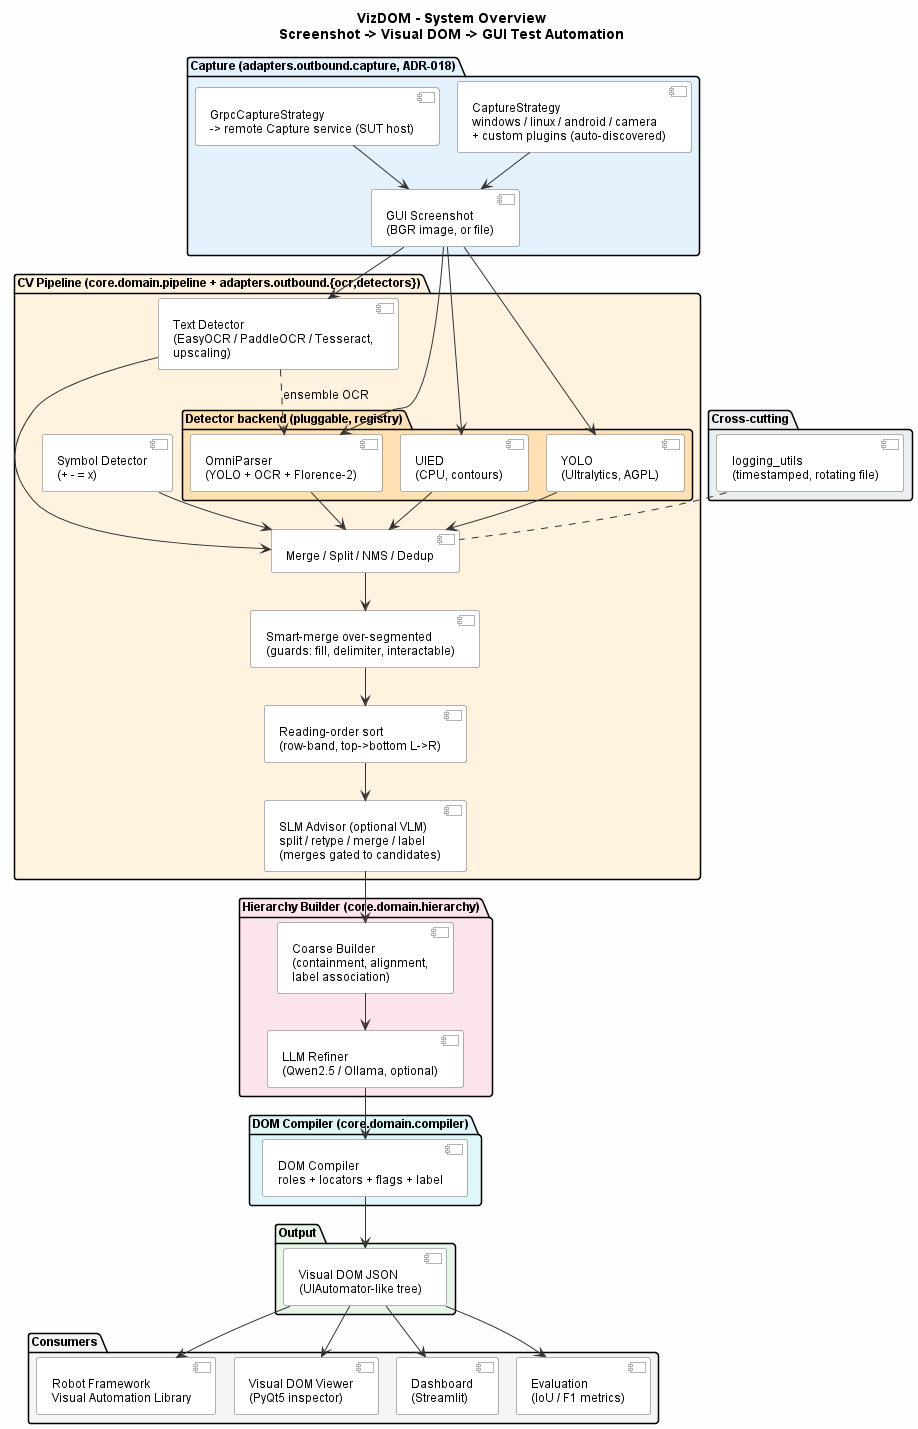
\includegraphics[width=0.6\linewidth]{System_Overview.png}
  \caption{Tổng quan và bối cảnh hệ thống. Biên trái: screenshot từ bất kỳ nguồn
  capture nào. Biên phải: Visual DOM được Robot Framework, Viewer, dashboard và
  evaluation harness sử dụng. Chú giải: các package có màu là subsystem; các mũi tên
  biểu diễn luồng dữ liệu hoặc điều khiển.}
  \label{fig:overview}
\end{figure}

\section{Bối cảnh kỹ thuật (các interface)}
\begin{longtable}{@{}p{3.4cm}p{3.0cm}p{7.6cm}@{}}
\toprule
\textbf{Hệ thống lân cận} & \textbf{Hướng} & \textbf{Interface} \\
\midrule
\endhead
Application under test & vào & Screenshot (ảnh BGR) thông qua capture strategy; các input event thông qua actuator strategy. \\
OCR engine & ra & EasyOCR~\cite{easyocr} / PaddleOCR / Tesseract~\cite{tesseract} dưới dạng thư viện in-process. \\
OmniParser & ra & Repository được vendor~\cite{omniparser2024} cùng weight Florence-2~\cite{florence2} / YOLO~\cite{ultralytics} lưu cục bộ. \\
Ollama & ra & HTTP đến small LM/VLM cục bộ hoặc từ xa để refinement tùy chọn. \\
Các dịch vụ từ xa & hai chiều & gRPC~\cite{grpc}: detector (\code{:50051}), capture (\code{:50053}), actuator (\code{:50054}). \\
Robot Framework & vào & Keyword library bằng Python~\cite{robotframework} sử dụng DOM. \\
\bottomrule
\end{longtable}

\section{Phạm vi}
\textbf{Trong phạm vi:} thu nhận screenshot, phát hiện phần tử/text, tổng hợp DOM,
phân giải locator, thực thi input, Robot Framework library và transport cho các dịch vụ
phân tán. \textbf{Ngoài phạm vi:} viết và lập lịch test case (do Robot Framework đảm
nhiệm), dịch vụ hosted multi-tenant, xác thực các kênh gRPC (được ghi nhận là technical
debt), và mọi thay đổi đối với application under test.

% =====================================================================
\chapter{Chiến lược Giải pháp}
% =====================================================================
\section{Tóm tắt chiến lược}
\begin{longtable}{@{}p{3.4cm}p{11.2cm}@{}}
\toprule
\textbf{Mục tiêu chất lượng} & \textbf{Cách tiếp cận kiến trúc} \\
\midrule
\endhead
Khả năng sửa đổi & \emph{Kiến trúc lục giác (ports \& adapters)}: domain core thuần chỉ phụ thuộc vào các port trừu tượng (Detector, Ocr, Refiner, Capture, Actuator). Mỗi port dùng mẫu \emph{strategy + registry + auto-discovery}, nhờ đó backend được bổ sung dưới dạng plugin. \\
Khả năng triển khai & Mỗi driven port có cả adapter in-process và gRPC client adapter; một gRPC server tương ứng bao bọc registry trên remote host. Transport là lựa chọn cấu hình riêng cho từng port, không đòi hỏi viết lại hệ thống. \\
Hiệu năng & Các model service được giữ \emph{warm}: model nặng chỉ tải một lần và phục vụ nhiều client nhẹ, qua đó phân bổ chi phí tải model cho nhiều request. \\
Khả năng kiểm thử & Core không phụ thuộc I/O mà chỉ phụ thuộc vào port; CPU detector không cần dependency đặc biệt (UIED), static-image capture và recording actuator cho phép chạy đầy đủ mà không cần GPU hoặc network. \\
Độ chính xác & Detector học máy có thể thay thế (OmniParser), kết hợp OCR ensemble và bước refinement bằng mô hình nhỏ có guard; UIED cổ điển đóng vai trò baseline. \\
\bottomrule
\end{longtable}

\section{Các driver được xếp hạng}
Bối cảnh: đây là một đồ án ứng dụng \emph{greenfield} với mục đích rõ ràng là mở rộng
trên nhiều detector và thiết bị; vì vậy khả năng sửa đổi và khả năng triển khai được xếp
cao hơn độ chính xác thuần túy. Nếu VizDOM là sản phẩm cố định cho một nền tảng duy nhất,
độ chính xác và độ tin cậy sẽ được xếp đầu tiên.

\begin{longtable}{@{}p{0.8cm}p{2.8cm}p{7.4cm}p{2.4cm}@{}}
\toprule
\textbf{Hạng} & \textbf{Driver} & \textbf{Diễn giải cụ thể} & \textbf{Loại} \\
\midrule
\endhead
\#1 & Khả năng sửa đổi & Thêm detector/capture/actuator mới mà không thay đổi core & Yêu cầu \\
\#2 & Khả năng triển khai & Port chạy in-process hoặc từ xa bằng cấu hình & Yêu cầu \\
\#3 & Khả năng kiểm thử & Chạy đầy đủ mà không cần GPU/network & Yêu cầu \\
\#4 & Độ chính xác & F1/IoU của detection trên UI thực tế & Yêu cầu \\
\#5 & Hiệu năng & Tái sử dụng warm model; độ trễ mỗi request chấp nhận được & Yêu cầu \\
-- & Hoạt động offline & Proxy chặn các public host, cần vendoring và tài liệu offline & Ràng buộc \\
-- & Không dùng container & Phân tán mà không dùng Docker/Nomad/Consul & Ràng buộc \\
\bottomrule
\end{longtable}

\paragraph{Xung đột giữa các driver.}
(a) \emph{Độ chính xác so với khả năng kiểm thử/khả năng di chuyển:} detector chính xác
nhất (OmniParser) cần GPU và các weight lớn, xung đột với yêu cầu ``chạy được trên laptop''.
Giải pháp là biến detector thành một port, có CPU baseline (UIED) và remote GPU service.
(b) \emph{Khả năng triển khai so với tính đơn giản:} các dịch vụ gRPC làm tăng số thành
phần vận hành; giải pháp là giữ gRPC ở dạng tùy chọn, còn in-process là mặc định.

\section{Quyết định chính: làm thế nào để detection/capture/actuation có thể mở rộng và triển khai linh hoạt}
Ba phương án được xem xét và chấm điểm theo các tiêu chí rút ra từ nhóm driver đã xếp hạng
(trọng số trong ngoặc): Khả năng sửa đổi~(5), Khả năng triển khai~(5), Khả năng kiểm
thử~(4), Độ phức tạp~(3, thấp hơn là tốt hơn), Độ phức tạp vận hành~(3, thấp hơn là tốt
hơn). Điểm số từ 1--5.

\begin{longtable}{@{}p{5.2cm}p{1.2cm}p{2.2cm}p{2.2cm}p{2.2cm}@{}}
\toprule
\textbf{Tiêu chí} & \textbf{Trọng số} & \textbf{A: hard-code theo từng consumer} & \textbf{B: shared library, chỉ in-process} & \textbf{C: strategy+registry + gRPC tùy chọn} \\
\midrule
\endhead
Khả năng sửa đổi & 5 & 1 (5) & 4 (20) & 5 (25) \\
Khả năng triển khai & 5 & 1 (5) & 2 (10) & 5 (25) \\
Khả năng kiểm thử & 4 & 2 (8) & 4 (16) & 5 (20) \\
Độ phức tạp (thấp hơn tốt hơn) & 3 & 4 (12) & 4 (12) & 2 (6) \\
Vận hành (thấp hơn tốt hơn) & 3 & 5 (15) & 4 (12) & 2 (6) \\
\midrule
\textbf{Tổng} & & \textbf{45} & \textbf{70} & \textbf{82} \\
\bottomrule
\end{longtable}

\textbf{Kết quả:} lựa chọn phương án~C. Phương án này vượt trội về khả năng sửa đổi và
khả năng triển khai, hai driver quan trọng nhất, đổi lại là độ phức tạp nội tại và vận hành
cao hơn. Đây là trade-off được chấp nhận rõ ràng và được giảm thiểu bằng cách giữ gRPC
ở dạng tùy chọn (hành vi của phương án~B là chế độ local mặc định), đồng thời dùng chung
một registry pattern cho cả ba port. Quyết định được ghi trong ADR-015 (detector), ADR-017
(gRPC phân tán), ADR-018 (capture) và ADR-019 (actuator).
Việc phân rã được định hướng có chủ đích theo \emph{microservice}: mỗi port là một
ranh giới dịch vụ độc lập, có hợp đồng protobuf được quản lý phiên bản và một server
có thể chạy riêng. Cách tổ chức này cho phép mở rộng quy mô độc lập (một detector dùng
warm GPU phục vụ nhiều client), triển khai trên các môi trường phần cứng khác nhau và
cô lập lỗi; đồng thời, khi các thành phần có thể được đặt cùng nhau, các dịch vụ vẫn có
thể được gom vào một process duy nhất. Nhờ đó, việc phân tán có thể được áp dụng từng
bước thay vì trở thành yêu cầu bắt buộc ngay từ đầu.

Hai quyết định sau đó hoàn thiện giao diện phía client: một \emph{session configuration}
dạng JSON duy nhất điều khiển toàn bộ các stage thông qua \code{connect()} hoặc keyword
\code{Connect} của Robot Framework (ADR-020); và locator \code{desc=} phân giải mô tả
phần tử bằng ngôn ngữ tự nhiên thông qua chuỗi grounding phân tầng --- trước hết là
lexical matching mang tính xác định, tiếp theo là một small LM xử lý trên DOM, và tùy
chọn dùng vision model thông qua Set-of-Mark. Các từ chỉ vị trí được kiểm tra bằng
geometry và kết quả được cache theo từng màn hình (ADR-022).

\section{Bức tranh các detector (lý do cần một port có thể thay thế)}
Detector port phải hỗ trợ nhiều công nghệ rất khác nhau. Bảng~\ref{tab:models} so sánh
các hệ thống ứng viên~\cite{xie2020uied,omniparser2024,ariaui2024,elam7b,osworldg}.
Chúng được chia thành hai họ: \emph{parser}, liệt kê toàn bộ phần tử (UIED, OmniParser,
VizDOM), và \emph{grounder}, trả về một điểm duy nhất cho một chỉ dẫn bằng ngôn ngữ tự
nhiên (Aria-UI, ELAM-7B, Jedi). Chỉ parser phù hợp với mục tiêu tạo một cây hoàn chỉnh
của VizDOM; không hệ thống nào được so sánh xây dựng cấu trúc phân cấp, và đây chính là
lớp đóng góp của đồ án. Port có thể thay thế cho phép VizDOM sử dụng parser mạnh nhất
(OmniParser) làm backend, giữ CPU baseline (UIED) cho các test rig không có GPU, và thay
một detector AGPL bằng detector có giấy phép permissive mà không sửa pipeline --- đây là
lý do cụ thể cho ADR-015. OmniParser backend còn ánh xạ đầu ra thô \code{text}/\code{icon}
sang taxonomy role của VizDOM (\code{button} / \code{input\_field} / \code{checkbox})
bằng heuristic kết hợp interactability và geometry có xét resolution, nhờ đó DOM có thể
được lớp kiểm thử sử dụng trực tiếp. Bảng~\ref{tab:arc42typeacc} định lượng phép ánh xạ
này: việc khôi phục role từ interactability, geometry và caption của OmniParser đã nâng độ
chính xác phân loại loại phần tử trên các control có thể thao tác từ \textbf{0.09} lên
\textbf{0.87}.

\begin{table}[H]
  \centering\footnotesize
  \caption{Độ chính xác phân loại loại phần tử của OmniParser trên các control có thể
  thao tác đã được matching, qua hai giai đoạn cải thiện trên tập synthetic: ban đầu
  chỉ có text/icon, bản sửa thứ nhất dùng interactability + geometry, và phiên bản hiện
  tại bổ sung caption cùng ngưỡng width/aspect đã được tinh chỉnh.}
  \label{tab:arc42typeacc}
  \begin{tabular}{@{}lccc@{}}
    \toprule
    Loại GT & Ban đầu & Bản sửa thứ nhất & Hiện tại \\
    \midrule
    button       & 0.00 & 0.91 & 0.89 \\
    input\_field & 0.00 & 0.99 & 0.99 \\
    checkbox     & 0.00 & 0.12 & 0.55 \\
    icon         & 1.00$^\dagger$ & 0.00 & \textbf{0.89} \\
    \midrule
    actionable   & 0.09 & 0.73 & \textbf{0.87} \\
    \bottomrule
  \end{tabular}
\end{table}

\noindent{\footnotesize $^\dagger$Phép ánh xạ cũ gán mọi phần tử không phải text thành
\code{icon}, nên chỉ icon được tính đúng còn mọi role khác đều bằng 0 --- vì vậy DOM không
thể nhận diện đúng các phần tử có thể thao tác. Kết quả localisation không thay đổi; bảng này
chỉ đo \emph{loại phần tử}.}

\begin{table}[H]
  \centering\footnotesize
  \caption{Bức tranh các hệ thống hiểu GUI theo kết quả do tác giả công bố; ``n/v'' =
  giấy phép chưa được xác minh.}
  \label{tab:models}
  \begin{tabular}{@{}p{2.3cm}p{2.4cm}p{2.7cm}p{0.7cm}p{2.2cm}p{2.0cm}@{}}
    \toprule
    Hệ thống & Mô hình tiếp cận & Mức chi tiết đầu ra & GPU & Nền tảng / kích thước & Giấy phép \\
    \midrule
    VizDOM (đề xuất) & parser (CV + SLM) & cây DOM phân cấp & Không$^\ast$ & pipeline kết hợp & theo từng backend \\
    UIED & CV cổ điển & danh sách phần tử phẳng & Không & --- & nghiên cứu \\
    OmniParser V2 & detector + caption & bounding box phẳng có label + interactability & Có & YOLOv8 + Florence-2 & AGPL-3.0 / MIT \\
    Aria-UI & vision grounding & một điểm $[0,1000]$ & Có & Aria MoE (3.9B tham số hoạt động) & n/v \\
    ELAM-7B & grounding + đánh giá & điểm + PASSED/FAILED & Có & Molmo-7B-D (Qwen2-7B) & Apache-2.0 \\
    Jedi-3B/7B & vision grounding & một điểm & Có & 3B / 7B & n/v \\
    \bottomrule
  \end{tabular}\\[0.3em]
  {\footnotesize $^\ast$ Chạy CPU qua UIED backend; OmniParser backend cần GPU để đạt tốc độ thực tế.}
\end{table}

% =====================================================================
\chapter{Góc nhìn Khối Xây dựng}
% =====================================================================
\section{Cấp 1 --- whitebox của VizDOM}
\begin{longtable}{@{}p{3.8cm}p{10.8cm}@{}}
\toprule
\textbf{Khối xây dựng} & \textbf{Trách nhiệm} \\
\midrule
\endhead
\code{visual\_dom.core.domain} & Phần lõi của hexagon (thuần, không I/O): điều phối pipeline; hierarchy builder + LLM refiner tùy chọn; DOM compiler; schema; reading-order; \code{cvops} (phát hiện symbol/screen, image processing). \\
\code{visual\_dom.core.ports.\allowbreak outbound} & Các interface driven-port mà lõi phụ thuộc: \code{detector\_port}, \code{capture\_port}, \code{actuator\_port}. \\
\code{visual\_dom.adapters.\allowbreak outbound} & Hiện thực cụ thể của các port: \code{detectors} (UIED/YOLO/OmniParser/gRPC + registry), \code{ocr} (text detector), \code{refiner} (SLM advisor), \code{capture} và \code{actuator} (built-in + gRPC client + plugin người dùng). \\
\code{visual\_dom.adapters.\allowbreak inbound.grpc} & Driving adapter: các gRPC server detector, capture và actuator. \\
\code{visual\_dom.context} & Composition root --- \code{connect()} / \code{Session} nối adapter vào lõi từ một file cấu hình. \\
\code{visual\_dom} (config, generated, dùng chung) & \code{config} (VizDomConfig), \code{generated} (protobuf stub), \code{logging\_utils}; \code{evaluation} là harness nằm ngoài hexagon. \\
\code{visual\_gui\_library} & Robot Framework keyword library, đóng vai trò thin client trên capture + actuator. \\
tools & PyQt5 Viewer, Streamlit dashboard và công cụ annotation. \\
\bottomrule
\end{longtable}

\noindent Cây package cố ý phản chiếu ports \& adapters --- \code{core/} (domain +
ports) hướng vào trong, \code{adapters/} (inbound + outbound) hướng ra ngoài ---
nên bố cục thư mục \emph{chính là} kiến trúc. Một fitness test tự động
(\code{tests/architecture/test\_hexagon.py}) kiểm tra chiều phụ thuộc: nó fail nếu
\code{core/} phát sinh một import mới tới \code{adapters/}. Ngoại lệ hiện tại (được
ghi nhận) là pipeline trực tiếp khởi tạo các backend OCR/UIED/refiner; chúng sẽ được
gỡ khi các thành phần đó chuyển ra sau port.

\begin{figure}[H]
  \centering
  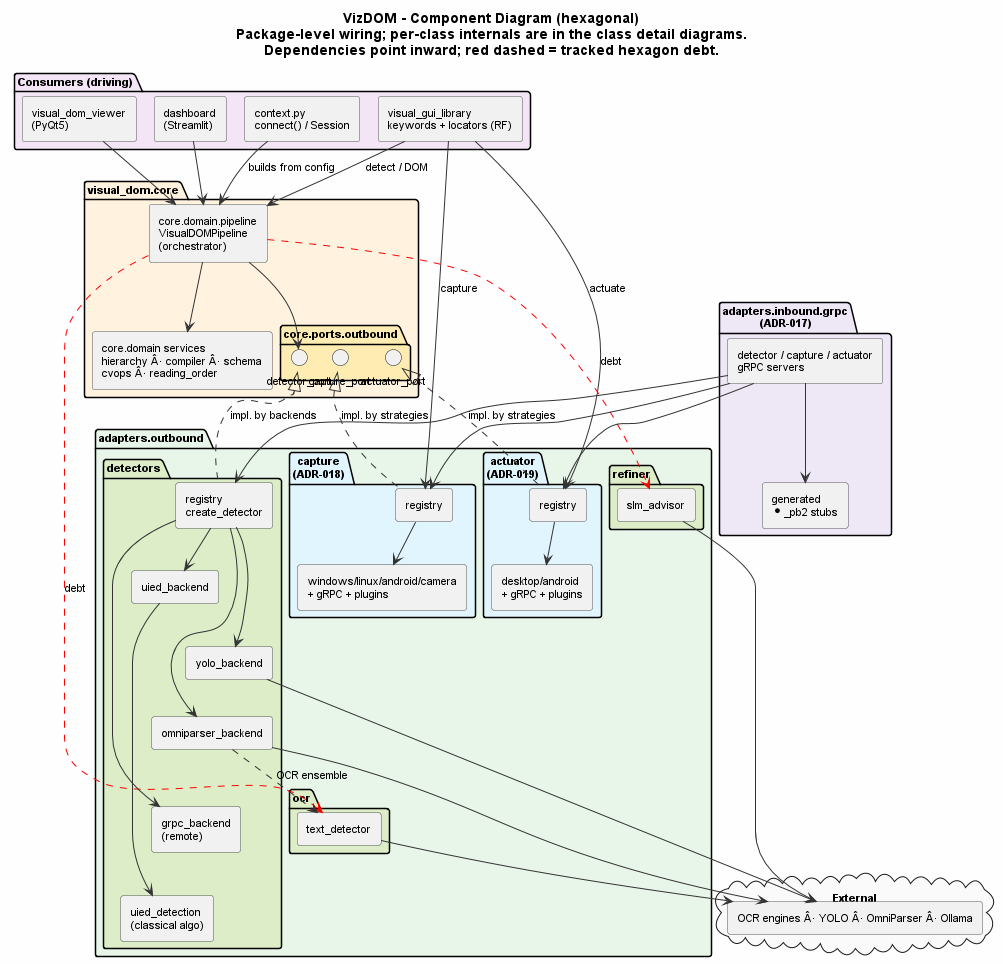
\includegraphics[width=\linewidth]{Component_Diagram.png}
  \caption{Các khối xây dựng cấp 1/2 và dependency giữa chúng. Chú giải: các hộp có
  màu là package; các hộp lồng nhau là subpackage; mũi tên biểu diễn ``phụ thuộc vào /
  gọi''. Biên hệ thống gồm mọi thành phần ngoại trừ đám mây \emph{External} gồm OCR
  engine, weight của OmniParser, Ollama và YOLO.}
  \label{fig:component}
\end{figure}

\section{Cấp 2 --- mẫu driven port}
Mỗi driven port (detector, capture, actuator) dùng chung một cấu trúc nội bộ:
\begin{itemize}[leftmargin=1.4em]
  \item Một \textbf{strategy base} với các abstract method, chẳng hạn \code{detect} /
        \code{capture} / \code{tap+type+swipe};
  \item Một \textbf{registry} cung cấp \code{create\_X(name)}, \code{list\_X()} và
        \code{auto\_select()};
  \item Cơ chế \textbf{auto-discovery} import các implementation tích hợp sẵn và mọi
        plugin người dùng được đặt trong thư mục quy ước;
  \item Một \textbf{gRPC client strategy} được đăng ký với tên \code{grpc}, nhờ đó
        remote adapter được lựa chọn giống hệt local adapter.
\end{itemize}
Việc lặp lại một mẫu duy nhất cho ba port là cơ chế hiện thực hóa NFR1 và NFR2.

\section{Cấp 2 --- thành phần nội bộ của CV pipeline}
Package \code{adapters.outbound.detectors} chứa tập hiện thực port
\code{DetectorBackend} --- một registry factory cùng các backend
UIED/YOLO/OmniParser/gRPC; \code{core.domain.pipeline} còn sở hữu các bước
merge/split/NMS, smart-merge, reading-order và SLM review (Ch.~6).

% =====================================================================
\chapter{Góc nhìn Runtime}
% =====================================================================
\section{Kịch bản 1 --- chuyển screenshot thành DOM cục bộ (happy path)}
Hình~\ref{fig:seq} mô tả một chu kỳ sử dụng OmniParser detector và bật SLM review.
Luồng chi tiết của pipeline được trình bày trong Hình~\ref{fig:pipeline}.

\begin{figure}[H]
  \centering
  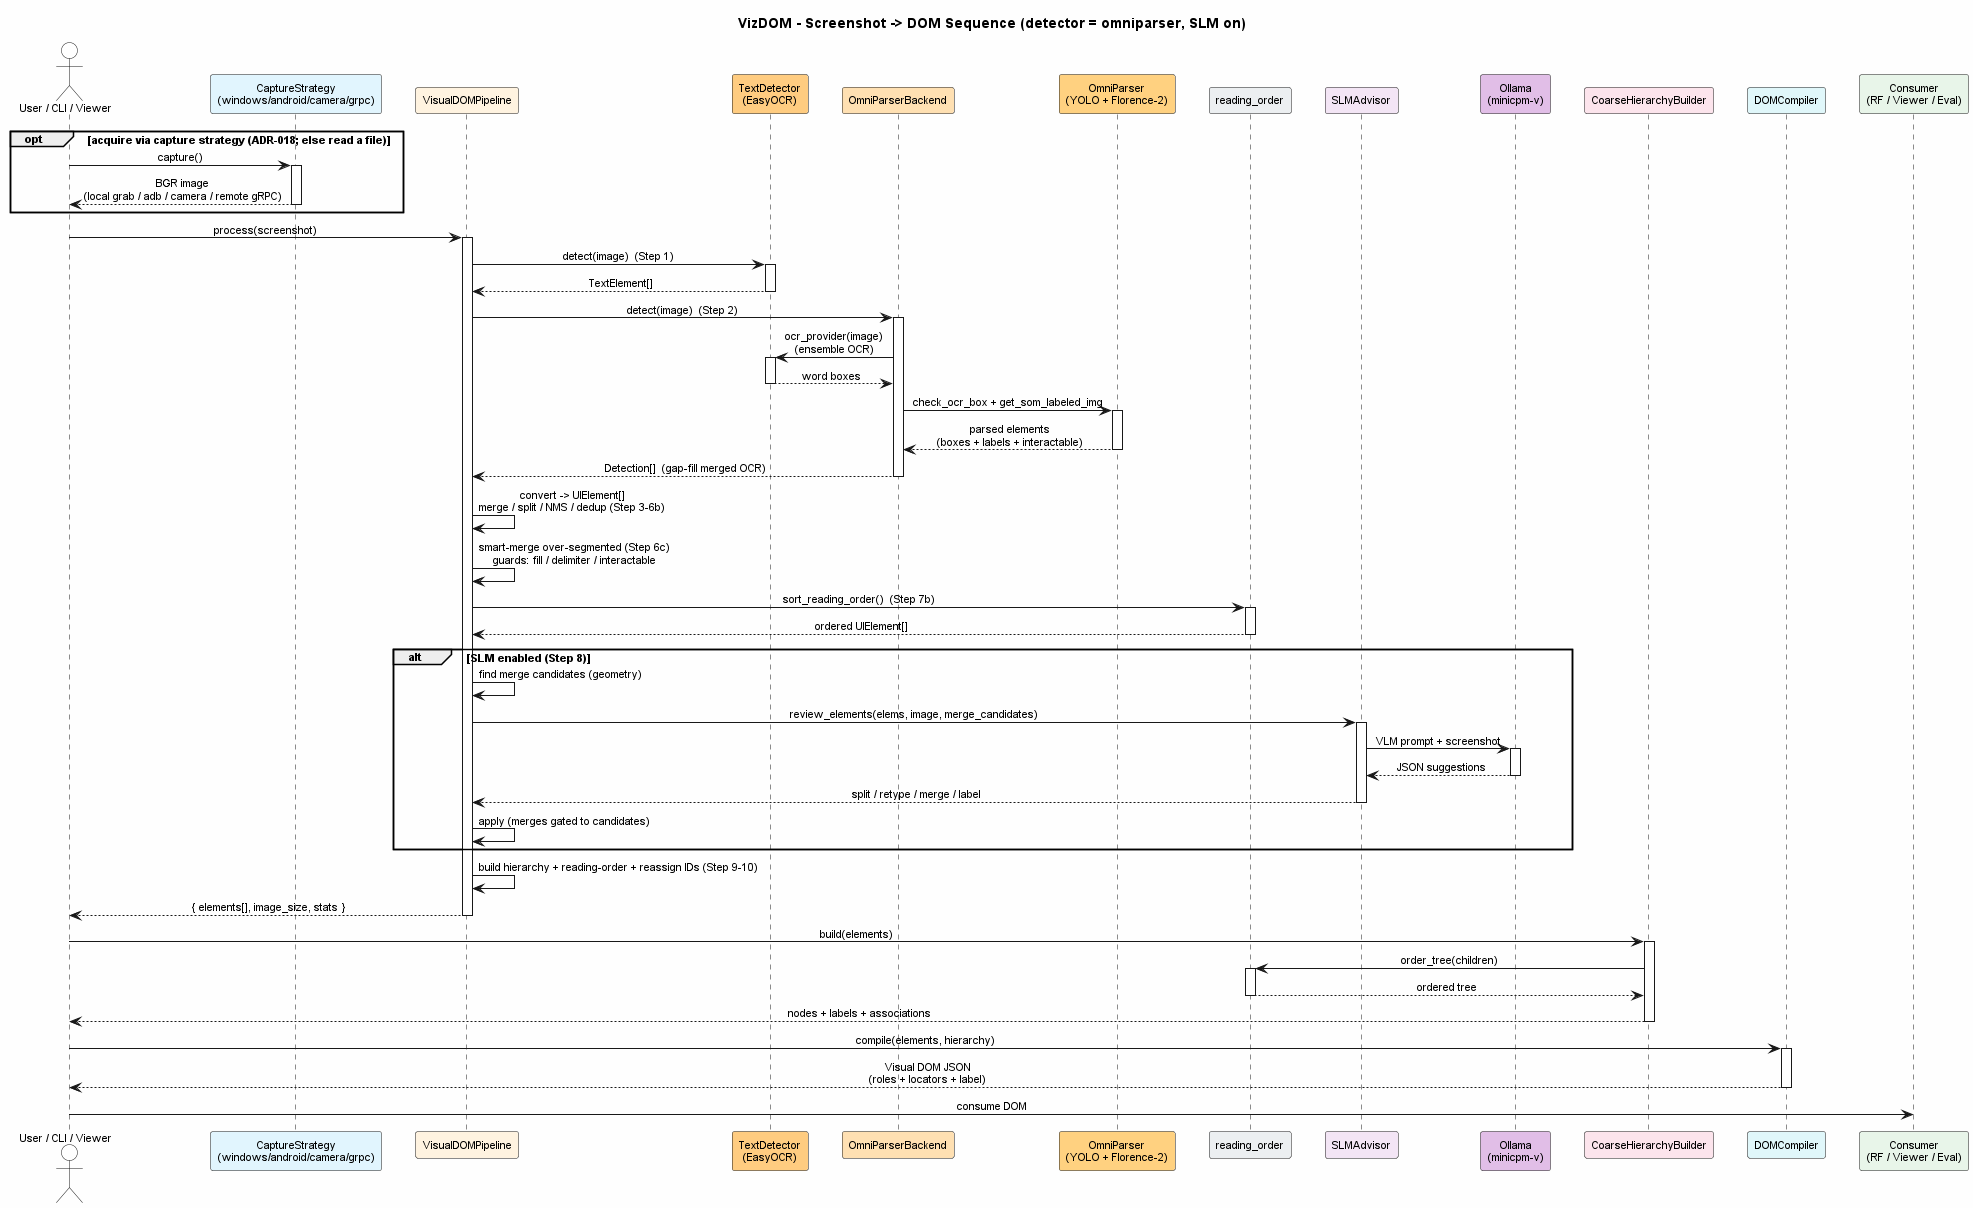
\includegraphics[width=\linewidth]{Sequence_Diagram.png}
  \caption{Kịch bản runtime 1: capture tùy chọn $\rightarrow$ OCR $\rightarrow$
  detection với OCR ensemble $\rightarrow$ clean-up $\rightarrow$ reading-order
  $\rightarrow$ SLM review tùy chọn $\rightarrow$ hierarchy $\rightarrow$ DOM.}
  \label{fig:seq}
\end{figure}

\begin{figure}[H]
  \centering
  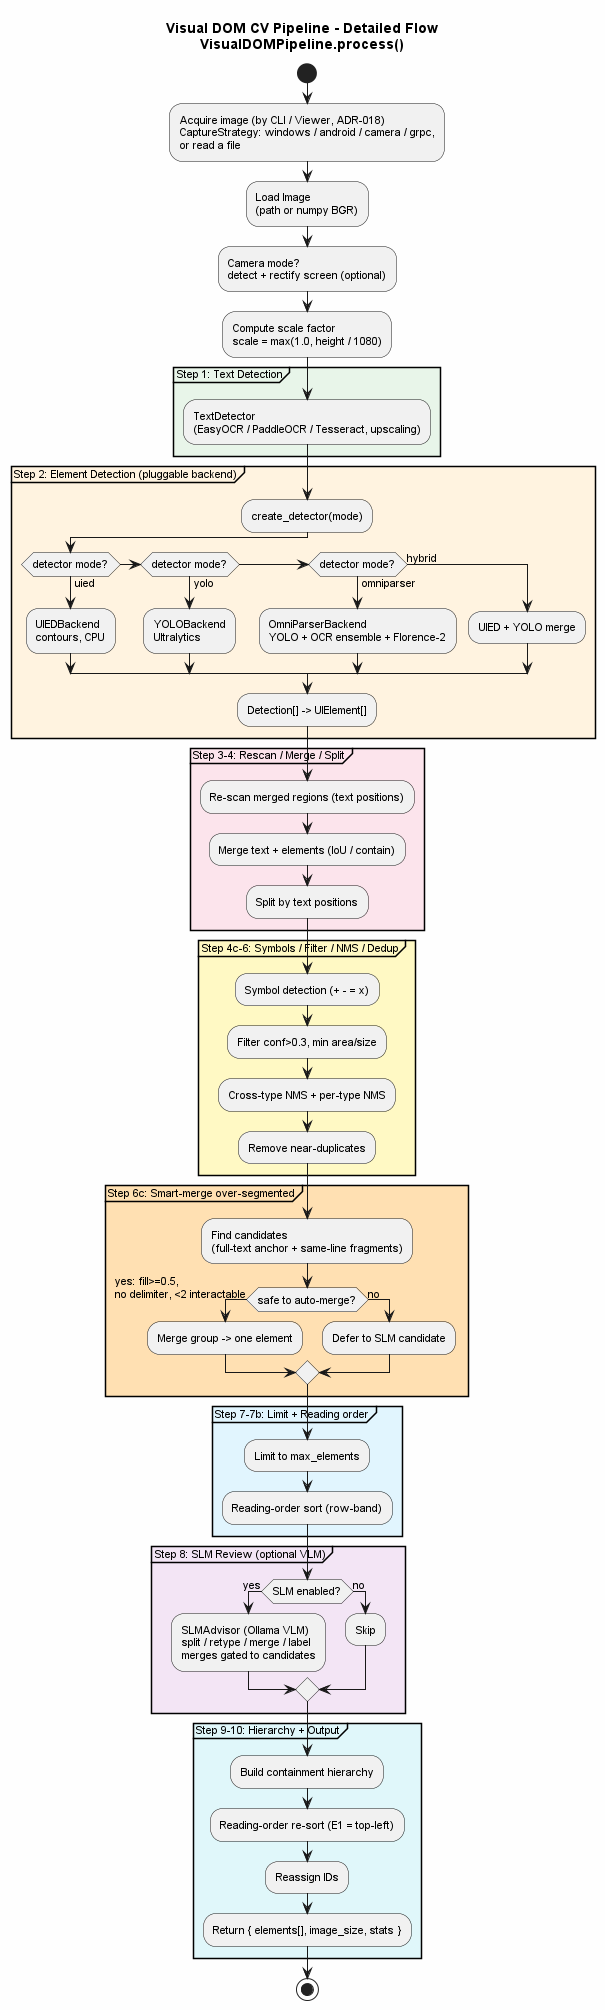
\includegraphics[height=0.82\textheight,width=\linewidth,keepaspectratio]{CV_Pipeline_Detail.png}
  \caption{Kịch bản runtime 1: luồng điều khiển chi tiết của
  \code{VisualDOMPipeline.process()}, bao gồm nhánh lựa chọn detector mode và các quyết
  định smart-merge / SLM có guard.}
  \label{fig:pipeline}
\end{figure}

\section{Kịch bản 2 --- capture, detect và actuate phân tán}
Một test run được điều phối trên client, trong khi capture chạy trên device under test
(\code{grpc} capture $\rightarrow$ capture service), detection chạy trên GPU host
(\code{grpc} detector $\rightarrow$ warm-model detector service), còn actuation chạy
trên thiết bị hoặc robot-arm controller (\code{grpc} actuator $\rightarrow$ actuator
service). Normalized coordinate được truyền qua actuator protocol và ánh xạ sang hệ tọa
độ của thiết bị ở phía server. Topology triển khai được trình bày trong
Hình~\ref{fig:arch}.

\section{Kịch bản 3 --- các luồng lỗi}
\begin{longtable}{@{}p{4.4cm}p{10.2cm}@{}}
\toprule
\textbf{Lỗi} & \textbf{Hành vi được thiết kế} \\
\midrule
\endhead
Không thể kết nối remote detector & Lời gọi gRPC client phát sinh exception; CLI/Viewer hiển thị lỗi. Biện pháp giảm thiểu/fallback: chọn UIED backend in-process bằng thay đổi cấu hình; backend này không cần GPU hoặc network. \\
Ảnh không hợp lệ được gửi đến service & Server xác thực input và trả về trạng thái \code{INVALID\_ARGUMENT}/\code{INTERNAL} kèm thông báo; server process vẫn tiếp tục chạy, một request lỗi không làm sập service. \\
Detector tạo quá nhiều phân đoạn & Rule-based smart-merge dựa trên fill-ratio / delimiter / interactable guard và guarded SLM merge sửa các phần tử bị phân mảnh; merge chỉ được phép trên các ứng viên đạt điều kiện geometry nên không hợp nhất các control riêng biệt. \\
OCR bỏ sót text & OCR ensemble đưa kết quả upscaling OCR của VizDOM vào OmniParser để khôi phục các từ bị bỏ sót bằng gap-fill deduplication. \\
SLM/Ollama không khả dụng & Refinement stage là tùy chọn; pipeline tiếp tục chỉ với kết quả CV. \\
\bottomrule
\end{longtable}

% =====================================================================
\chapter{Góc nhìn Triển khai}
% =====================================================================
\section{Môi trường phát triển / một máy}
Tất cả port chạy in-process trong cùng một Python process; không service nào được khởi
động. Đây là chế độ mặc định, đồng thời là chế độ dùng cho kiểm thử và đánh giá đồ án.

\section{Triển khai phân tán}
\begin{figure}[H]
  \centering
  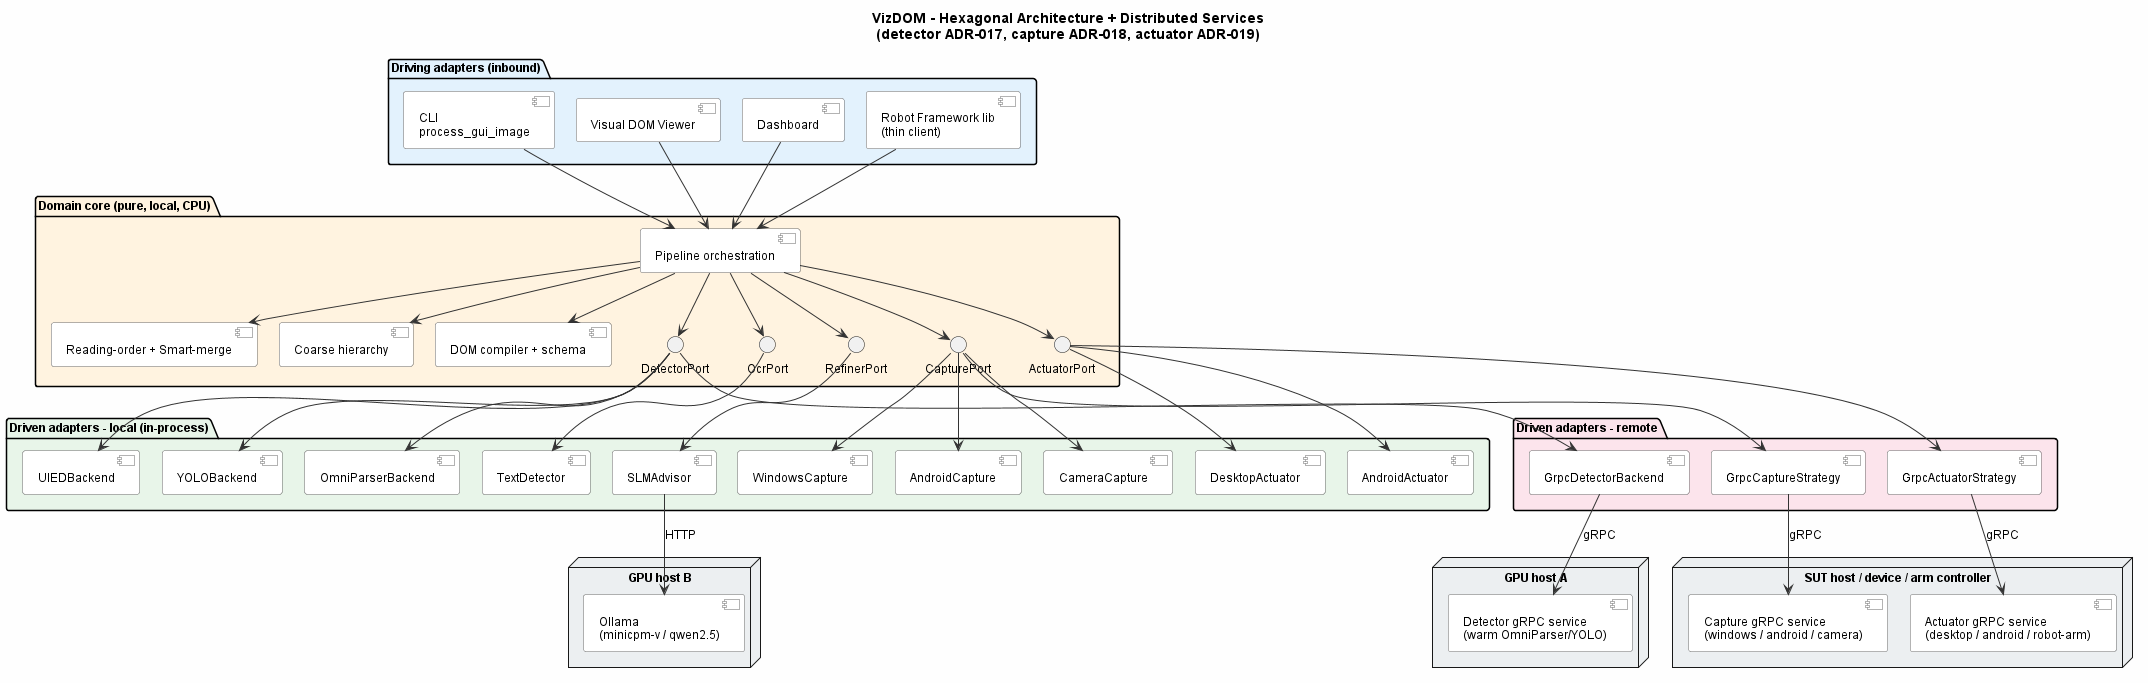
\includegraphics[width=\linewidth]{Architecture.png}
  \caption{Góc nhìn triển khai / ports-and-adapters. Driving adapter ở phía trên đi
  vào core; driven port ở dải giữa liên kết với local adapter hoặc remote gRPC adapter;
  các gRPC service chạy trên GPU host và SUT/robot-arm controller ở phía dưới. Chú giải:
  hộp bo góc là component; vòng tròn interface là port; hộp 3-D là deployment node;
  cạnh có nhãn gRPC/HTTP là network call.}
  \label{fig:arch}
\end{figure}

\begin{longtable}{@{}p{4.2cm}p{4.2cm}p{6.0cm}@{}}
\toprule
\textbf{Node} & \textbf{Thành phần chạy trên node} & \textbf{Ghi chú} \\
\midrule
\endhead
Client / orchestrator & CLI hoặc Robot Framework + domain core & Chọn các strategy \code{grpc}; không chứa model nặng. \\
GPU host & Detector gRPC service & Warm OmniParser/YOLO; \code{:50051}. \\
SUT host / thiết bị & Capture + Actuator gRPC service & \code{:50053} / \code{:50054}; nơi application under test chạy. \\
Robot-arm controller & Actuator gRPC service với robot-arm plugin & Áp dụng phép calibration từ ảnh sang tọa độ vật lý. \\
LM host & Ollama & HTTP; dùng cho refinement tùy chọn. \\
\bottomrule
\end{longtable}

Khả năng quan sát: dùng chung rotating file logger (\code{logging\_utils}), gắn correlation
ID cho từng gRPC request; mỗi service ghi log thời gian xử lý theo request.

% =====================================================================
\chapter{Các Khái niệm Xuyên suốt}
% =====================================================================
\begin{description}[leftmargin=0pt,style=nextline]
  \item[Khả năng mở rộng (strategy + registry + auto-discovery)] Đây là khái niệm quan
    trọng nhất; xem Ch.~5. Một plugin là một file kế thừa strategy base và được tự động
    tải theo tên. \emph{Lưu ý bảo mật:} discovery thực hiện import mã plugin --- chỉ sử
    dụng plugin đáng tin cậy.
  \item[Hợp đồng normalized coordinate] Các action của actuator dùng tọa độ trong
    $[0,1]$ cùng kích thước ảnh nguồn; mỗi thiết bị ánh xạ sang không gian riêng
    (desktop nhân theo độ phân giải màn hình, Android nhân theo input resolution,
    robot arm dùng homography). Cơ chế này giữ orchestrator và wire protocol độc lập
    với độ phân giải.
  \item[Warm-model service] Model nặng chỉ được tải một lần trong mỗi service process;
    client là stateless và nhẹ.
  \item[Xử lý lỗi] Service không bị sập bởi một request lỗi; service trả về gRPC status
    và tiếp tục phục vụ. Các bước tùy chọn như SLM và refiner được graceful degradation.
  \item[Cấu hình] Strategy được lựa chọn theo tên từ CLI flag, library argument hoặc
    environment variable; target cho remote port là chuỗi host:port.
  \item[Lưu trữ] Kết quả phân tích được ghi vào session folder có timestamp, gồm
    screenshot, kết quả CV, DOM và metadata.
  \item[Giấy phép] Nghĩa vụ AGPL được áp dụng khi OmniParser backend được cung cấp qua
    network; UIED là phương án fallback không chịu AGPL.
  \item[Hoạt động offline] Mã model bên ngoài được vendor và \emph{pin} bằng setup
    script; tài liệu render UML offline từ file jar được vendor sẵn.
\end{description}

% =====================================================================
\chapter{Các Quyết định Kiến trúc}
% =====================================================================
Các quyết định được ghi dưới dạng ADR trong \code{docs/adr/}. Danh sách các quyết định
có ý nghĩa kiến trúc cùng trạng thái hiện tại được trình bày dưới đây; lưu ý ADR-017 vẫn
đang ở trạng thái \emph{Proposed}, đây là một lưu ý khi xác minh ở Ch.~11.

\begin{longtable}{@{}p{1.4cm}p{7.8cm}p{2.4cm}@{}}
\toprule
\textbf{ADR} & \textbf{Quyết định} & \textbf{Trạng thái} \\
\midrule
\endhead
015 & Detector backend có thể thay thế (UIED/YOLO/OmniParser) & Đã chấp thuận \\
016 & Sắp xếp reading order và label phần tử & Đã chấp thuận \\
017 & Kiến trúc lục giác phân tán với gRPC model service & \textbf{Đề xuất} \\
018 & Screenshot capture có thể thay thế (strategy + service) & Đã chấp thuận \\
019 & Input actuation có thể thay thế (strategy + service) & Đã chấp thuận \\
020 & Cấu hình phiên phía client (\code{connect} + một file JSON cho toàn bộ các stage) & Đã chấp thuận \\
022 & Locator dựa trên mô tả (\code{desc=}) thông qua grounding phân tầng (lexical $\rightarrow$ SLM-over-DOM $\rightarrow$ VLM Set-of-Mark) & Đã chấp thuận \\
\bottomrule
\end{longtable}

\section{ADR mẫu (rút gọn): ADR-019 --- Input actuation có thể thay thế}
\textbf{Bối cảnh.} Input actuation trước đây nằm trong các Robot Framework adapter,
làm trùng lặp capture và không tạo điểm mở rộng cho plugin, chẳng hạn robot arm.
\textbf{Driver.} NFR1 (khả năng sửa đổi), NFR2 (khả năng triển khai).
\textbf{Quyết định.} Giới thiệu \code{ActuatorPort} --- thành phần phía ghi tương ứng
với \code{CapturePort} --- gồm strategy base, registry có auto-discovery, các
implementation tích hợp sẵn được chuyển khỏi RF adapter, hợp đồng normalized coordinate
và gRPC service tùy chọn. \textbf{Phương án thay thế.} (a) giữ input trong RF: không có
điểm mở rộng và capture tiếp tục bị trùng lặp; (b) actuator API ở cấp element: kéo kiến
thức về DOM xuống device layer; (c) truyền absolute pixel: buộc orchestrator phải biết
độ phân giải của từng thiết bị. \textbf{Hệ quả.} Loại bỏ trùng lặp; robot arm, capture
card hoặc serial device có thể được tích hợp bằng plugin một file; RF library trở thành
thin client. Trade-off: calibration từ ảnh sang không gian vật lý là công việc thực tế
và được cô lập trong plugin; physical actuation kéo theo các nghĩa vụ an toàn mà plugin
phải bảo đảm.

% =====================================================================
\chapter{Các Yêu cầu Chất lượng}
% =====================================================================
\section{Cây chất lượng (các thuộc tính chính)}
Khả năng sửa đổi và khả năng triển khai là hai gốc của cây chất lượng theo nhóm driver
được xếp hạng, tiếp theo là khả năng kiểm thử, sau đó đến độ chính xác và hiệu năng.

\section{Các kịch bản thuộc tính chất lượng}
\begin{longtable}{@{}p{2.2cm}p{12.4cm}@{}}
\toprule
\multicolumn{2}{@{}l}{\textbf{Q-01 --- Khả năng sửa đổi}} \\
\midrule
\endfirsthead
Driver & Bổ sung một detection backend mới. \\
Kích thích & Developer cần một detector mới, chẳng hạn một grounding model khác. \\
Môi trường & Giai đoạn phát triển; core hiện có không thay đổi. \\
Artifact & Registry \code{visual\_dom.cv.detectors} + một file backend mới. \\
Phản hồi & Backend được phát hiện và có thể lựa chọn theo tên. \\
Thước đo phản hồi & 1 file mới + 1 dòng registry; \textbf{0} chỉnh sửa core; port có $\geq 2$ implementation, hiện tại là 4: UIED/YOLO/OmniParser/gRPC. \\
\bottomrule
\end{longtable}

\begin{longtable}{@{}p{2.2cm}p{12.4cm}@{}}
\toprule
\multicolumn{2}{@{}l}{\textbf{Q-02 --- Khả năng triển khai}} \\
\midrule
\endhead
Kích thích & Di chuyển capture sang thiết bị và detection sang GPU host. \\
Môi trường & Ba máy trong cùng LAN. \\
Artifact & Capture/detector port + gRPC service. \\
Phản hồi & Cùng một orchestration tiếp tục chạy bằng cách chọn strategy \code{grpc}. \\
Thước đo phản hồi & Chỉ thay đổi cấu hình gồm tên strategy và host:port; \textbf{0} thay đổi code; round-trip end-to-end thành công. \\
\bottomrule
\end{longtable}

\begin{longtable}{@{}p{2.2cm}p{12.4cm}@{}}
\toprule
\multicolumn{2}{@{}l}{\textbf{Q-03 --- Hiệu năng (warm model)}} \\
\midrule
\endhead
Kích thích & Client gửi liên tiếp nhiều detection request. \\
Môi trường & Detector service chạy trên GPU host. \\
Artifact & Detector gRPC service. \\
Phản hồi & Model được tải một lần và được tái sử dụng. \\
Thước đo phản hồi & Model chỉ được tải đúng một lần trong vòng đời service; các request tiếp theo chỉ chịu chi phí inference. \\
\bottomrule
\end{longtable}

\begin{longtable}{@{}p{2.2cm}p{12.4cm}@{}}
\toprule
\multicolumn{2}{@{}l}{\textbf{Q-04 --- Khả năng kiểm thử}} \\
\midrule
\endhead
Kích thích & Chạy toàn bộ pipeline và RF keyword trong CI trên laptop. \\
Môi trường & Không GPU, không network. \\
Artifact & Core + UIED + static-image capture + recording actuator. \\
Phản hồi & DOM được tạo và keyword thực hiện action mà không cần I/O thật. \\
Thước đo phản hồi & Full run hoàn tất mà không phụ thuộc GPU/network. \\
\bottomrule
\end{longtable}

\begin{longtable}{@{}p{2.2cm}p{12.4cm}@{}}
\toprule
\multicolumn{2}{@{}l}{\textbf{Q-05 --- Độ chính xác}} \\
\midrule
\endhead
Kích thích & Phát hiện phần tử trên các UI đại diện. \\
Môi trường & Benchmark dataset có gán nhãn. \\
Artifact & Detector + clean-up + refinement. \\
Phản hồi & Detection khớp với ground truth. \\
Thước đo phản hồi & Mục tiêu F1 $\geq 0.80$, mIoU $\geq 0.60$. \emph{Kết quả đo trên tập synthetic gồm 44 ảnh, tính gộp:} F1 $0.51$ (UIED) / $0.58$ (OmniParser); chưa đạt mục tiêu F1, đạt mục tiêu mIoU (0.67--0.68). Recall trên actionable control với IoU$\geq$0.5: OmniParser button 1.00, input 0.99, icon 0.67; UIED button 0.82, input 0.95, checkbox 0.68. Click-targetability theo center-hit: OmniParser 0.97, UIED 0.89. \\
\bottomrule
\end{longtable}

\section{Kế hoạch xác minh}
\begin{longtable}{@{}p{2.0cm}p{5.4cm}p{4.4cm}p{2.2cm}@{}}
\toprule
\textbf{Kịch bản} & \textbf{Cách xác minh} & \textbf{Tiêu chí chấp nhận} & \textbf{Trạng thái} \\
\midrule
\endhead
Q-01 & Đếm implementation trên từng port; thêm một backend trong test & $\geq 2$ implementation; 0 chỉnh sửa core & \textbf{Đã xác minh} (4 detector, 5 capture, 3 actuator) \\
Q-02 & Round-trip gRPC end-to-end qua nhiều process & chỉ thay đổi cấu hình; round-trip thành công & \textbf{Đã xác minh về chức năng} (capture cho ảnh giống hệt theo pixel; actuator mapping chính xác; detector tái sử dụng warm model) \\
Q-03 & Instrument số lần tải model trong service & số lần tải = 1 & \textbf{Đã xác minh về chức năng} \\
Q-04 & Chạy pipeline + RF với CPU/static/recording adapter & hoàn tất, không I/O thật & \textbf{Đã xác minh} \\
Q-05 & Đo detection metric trên tập synthetic bằng evaluation harness & F1 $\geq 0.80$, mIoU $\geq 0.60$ & \textbf{Đã đo}: F1 0.58, mIoU 0.68; chưa đạt mục tiêu F1; actionable center-hit của OmniParser đạt 0.97 (R-04) \\
\bottomrule
\end{longtable}

% =====================================================================
\chapter{Rủi ro và Nợ Kỹ thuật}
% =====================================================================
\begin{longtable}{@{}p{1.2cm}p{5.0cm}p{2.0cm}p{5.6cm}@{}}
\toprule
\textbf{ID} & \textbf{Rủi ro / Nợ kỹ thuật} & \textbf{Tác động / Khả năng xảy ra} & \textbf{Biện pháp giảm thiểu} \\
\midrule
\endhead
R-01 & ADR-017 về gRPC phân tán đang ở trạng thái \emph{Proposed}, nhưng bằng chứng cho NFR2 lại dựa trên quyết định này & Cao / -- & Chấp thuận ADR-017 sau khi review, hoặc hạ mức tuyên bố về khả năng triển khai thành ``đã chứng minh, chưa được phê chuẩn''. \\
R-02 & Các kênh gRPC chưa được xác thực hoặc mã hóa & Cao / Trung bình & Hiện chỉ dùng trong LAN; bổ sung TLS + authentication trong hạng mục tiếp theo. \\
R-03 & Plugin auto-discovery thực thi code của người dùng; actuator có thể điều khiển robot arm vật lý & Cao / Thấp & Chính sách chỉ dùng plugin đáng tin cậy; ghi rõ an toàn như giới hạn vùng hoạt động và e-stop là trách nhiệm của plugin. \\
R-04 & F1 tổng hợp dựa trên IoU thấp hơn mục tiêu (0.58 so với 0.80); một metric IoU duy nhất che khuất việc cả hai detector đều xác định click target tốt & Trung bình / Cao & Báo cáo center-hit cùng IoU; bổ sung tập dữ liệu thực tế có gán nhãn; xem xét lại liệu mục tiêu F1 0.80 có phải mục tiêu vận hành phù hợp hay không. \\
R-05 & Over-segmentation trên UI thực tế có nhiều gradient & Trung bình / Trung bình & Smart-merge + guarded SLM; tiếp tục tinh chỉnh. \\
D-01 & Metric hiện chỉ bao phủ element detection + OCR vì ground truth chưa có tree / locator & Thấp / -- & Các trục hierarchy + locator cần ground truth có cấu trúc cây. \\
D-02 & Code registry/discovery bị lặp lại trên ba port & Thấp / -- & Tách một plugin-registry base dùng chung. \\
\bottomrule
\end{longtable}

\section{Kết quả D-CAR (review tập trung vào quyết định)}
\begin{longtable}{@{}p{4.6cm}p{5.0cm}p{4.4cm}@{}}
\toprule
\textbf{Quan sát} & \textbf{Ảnh hưởng} & \textbf{Hành động} \\
\midrule
\endhead
NFR2 truy vết đến ADR-017, nhưng ADR này đang ở trạng thái \emph{Proposed} thay vì \emph{Accepted}. & Tuyên bố gắn với một driver quan trọng dựa trên quyết định chưa được phê chuẩn. & Phê chuẩn ADR-017 hoặc diễn đạt lại rằng khả năng này mới được chứng minh. (R-01) \\
Cơ chế phân tán đã được triển khai nhưng quyết định bảo mật còn ngầm định: dùng kênh không an toàn và chưa có ADR. & Quyết định bị ẩn; reviewer không nhìn thấy trade-off. & Viết ADR cho transport security và bổ sung TLS. (R-02) \\
Khả năng sửa đổi vừa được tuyên bố, vừa được chứng minh bằng số implementation 4/5/3. & Tuyên bố mạnh và có thể xác minh. & Tiếp tục tự động cập nhật số implementation từ repository. \\
F1 tại IoU$\geq$0.5 là 0.58, thấp hơn mục tiêu, nhưng center-hit cho thấy cả hai detector đều định vị tốt actionable control (OmniParser 0.97, UIED 0.89). & Một metric IoU duy nhất đánh giá thấp tính hữu dụng trong vận hành. & Báo cáo center-hit cùng IoU; bổ sung tập dữ liệu thực tế; xem xét lại mục tiêu F1. (R-04) \\
\bottomrule
\end{longtable}

% =====================================================================
\chapter{Bảng Thuật ngữ}
% =====================================================================
\begin{longtable}{@{}p{3.8cm}p{10.8cm}@{}}
\toprule
\textbf{Thuật ngữ} & \textbf{Định nghĩa} \\
\midrule
\endhead
Visual DOM & Cây JSON tương tự UI Automator gồm bounds, role, text, label, locator và hierarchy, được tổng hợp từ screenshot. \\
Port / Adapter & Biên dependency trừu tượng (port) và implementation cụ thể của nó (adapter), theo kiến trúc lục giác. \\
Driven port & Port được core \emph{gọi}, gồm Detector, Ocr, Refiner, Capture và Actuator. \\
Strategy & Implementation có thể thay thế, được lựa chọn theo tên tại runtime. \\
Registry & Cơ chế factory + discovery dùng để tìm và khởi tạo strategy. \\
Warm model & Model được giữ trong trạng thái đã tải bên trong service process sống lâu để phân bổ chi phí tải model cho nhiều request. \\
Normalized coordinate & Tọa độ trong $[0,1]$ theo chiều rộng/chiều cao ảnh, được mỗi actuator ánh xạ sang không gian thiết bị. \\
UIED & CPU element detector cổ điển, không yêu cầu dependency đặc biệt, dùng làm baseline~\cite{xie2020uied}. \\
OmniParser & Detector học máy: YOLO icon detection + caption Florence-2 + OCR. \\
SLM / VLM & Small language model / vision-language model được dùng để review phần tử ở bước tùy chọn. \\
Homography & Phép biến đổi chiếu $3\times3$ từ pixel ảnh sang tọa độ vật lý, dùng để calibration robot arm. \\
\bottomrule
\end{longtable}

\bibliographystyle{plain}
\bibliography{references}

\end{document}
